
\documentclass[10pt,openany,a4paper]{article}
\usepackage{tikz, pgfplots, tkz-euclide,calc}
\usetikzlibrary{patterns,shapes.arrows,calc}
\usepackage{fancyhdr}
\usepackage{enumerate,enumitem}
\usepackage{cancel}
\usepackage{varwidth}

% TAMBAHKAN PACKAGE SENDIRI KALAU KURANG

\usepackage{geometry}
\geometry{
	left = 22mm,
	right = 22mm,
	top = 25mm,
	bottom = 25mm,
}
\usepackage{graphicx}
\usepackage{subcaption}
\usepackage{soul}
\usepackage{hyperref}
\usepackage{float}
\usepackage{setspace}
\usepackage{afterpage}
\usepackage{xcolor}
\usepackage[nosectionbib]{apacite}
\usepackage{lmodern}
\usepackage{mathtools}
\usepackage{upgreek}
\usepackage{siunitx}
% \usepackage{fontawesome5}
\usepackage{fontawesome6}
\usepackage{physics}
\usepackage{pdfpages}
\usepackage{hyperref}
\renewcommand{\baselinestretch}{1.3}
\usepackage{multicol}
\usepackage{hyperref,ragged2e,amsmath,multicol,gensymb,setspace,
fancyhdr,amsfonts,tikz,pgfplots,nccmath,enumerate,verbatim,amsthm,physics}
\usepgfplotslibrary{polar,fillbetween}
% Disable tikz externalization to avoid requiring -shell-escape
\usepgfplotslibrary{external}
\tikzexternalize[prefix=tikz/]
\tikzset{reuse path/.code={\pgfsyssoftpath@setcurrentpath{#1}}}
\usetikzlibrary{shapes.geometric,arrows}
\newcommand\mylog[1]{\mathop{{}^{#1}\mathrm{log}}}
\pgfplotsset{compat=1.15}
\pgfplotsset{my style/.append style={axis x line=middle, axis y line=
middle, xlabel={$x$}, ylabel={$y$}, axis equal }}
\usepackage{etoolbox}
% remove stray \makeatother
\newtheorem{defn}{Definisi}[section]
\newtheorem{teo}[defn]{Teorema}
\newtheorem{thm}{Teorema}[section]
\newtheorem{lemma}{Lemma}
\newtheorem{lemmas}[defn]{Lemma}
\newtheorem{cor}[defn]{Akibat}
\newtheorem{asumsi}[defn]{Asumsi}
\theoremstyle{definition}
\newtheorem{con}{Contoh}[section]
\theoremstyle{definition}
\theoremstyle{plain}
\newtheorem{prop}{Proposisi}[section]
\renewcommand{\proofname}{Bukti}
\renewcommand{\thethm}{\arabic{chapter}.\arabic{thm}}

\newcommand{\normlp}[1]{\left\|#1\right\|_{L^p_{\lambda}(0,T;H)}}% Fungsi norm (||x||)
\newcommand{\R}{\mathbb{R}}
\renewcommand{\natural}{\mathbb{N}}
\newcommand{\Xpl}{X^R_{p,\lambda}}
\newcommand{\Xpls}{X^R_{p,\lambda^*}}
\newcommand{\qpl}{q^R_{p,\lambda}}
\newcommand{\qpls}{q^R_{p,\lambda^*}}
\pagestyle{fancy}
\fancyhf{}
\lhead{Halaman \thepage}
% \cfoot{\faXTwitter\ \href{https://x.com/ahmadzakiyudin_/}{@ahmadzakiyudin\_} | \faInstagram\ \href{https://instagram.com/ahmadzakiyudin_/}{@ahmadzakiyudin\_} | \faTiktok\ \href{https://tiktok.com/@ahmathz/}{@ahmathz}}
% \rhead{Pembahasan Soal ETS \\ Kalkulus 1 ITS 2025/2026}
\hypersetup{
    colorlinks=true,
    linkcolor=blue,
    filecolor=blue,      
    urlcolor=blue,
}
\newenvironment{jawab}[2][tes]{
% \fbox{\begin{minipage}{14.65cm}
\textbf{Kata kunci materi:} #1.\\
\textbf{Penyelesaian:} #2
% \end{minipage}}
}{}

\newenvironment{jawab2}[2][tes]{
\fbox{\begin{minipage}{14.65cm}
 #2
\end{minipage}}}{}

\newenvironment{jawaban}[2][tes]{
\colorlet{oldcolor}{.}
        \color{red}
        \setlength{\fboxrule}{1pt}\boxed{\color{oldcolor}#2}\color{oldcolor}.
}{}

\newenvironment{jawaban2}[2][tes]{
\colorlet{oldcolor}{.}
        \color{red}
        \setlength{\fboxrule}{1pt}\fbox{\color{oldcolor}#2}\color{oldcolor}.
}{}

\newenvironment{penting}[2][tes]{
\colorlet{oldcolor}{.}
\color{blue}
\fbox{\color{oldcolor}#2}\color{oldcolor}
}{}

\begin{document}
% \begin{titlepage}
%     \vspace*{\fill}
%     \begin{center}
%       \Huge {PEMBAHASAN SOAL EAS \\ KALKULUS II \\ TAHUN 2024/2025}\\[0.4 cm]
%       \huge {Ahmad Hisbu Zakiyudin}\\[0.2 cm]
%       \Large {(\href{https://instagram.com/ahmadzakiyudin_/}{@ahmadzakiyudin\_})}
%     \end{center}
%     \vspace*{\fill}
%   \end{titlepage}
% !TEX root = ../../BookTemplate.tex
%%%%%%%%%%%%%%%%%%%%%%%%%%%%%%%%%%%%%%%%%%%%%%%%%%%%%%%%%%%%%%%%%%%%%%%%%%%%%%%%%%
% \begin{titlepage}
%     \raggedleft	
% 	\hspace{.025\textwidth}
% 	\parbox[b]{\textwidth}{
%     \vspace{1.5cm}
% 		{\Huge\bfseries Pembahasan Soal EAS}                \\[20pt]
% 		{\huge\textit\ Kalkulus II}\\ \\[10pt]
%         {\Large\textsc{Tahun 2024/2025}}}
% \vfill
% \rule{1pt}{.14\textheight}
% \hspace{.025\textwidth}
%     \raisebox{10pt}{\parbox[b]{.95\textwidth}{ 
%         {\Large\textsc{Ahmad Hisbu Zakiyudin}}              \\[10pt]
%         \large{\href{https://instagram.com/ahmadzakiyudin_/}{@ahmadzakiyudin\_}}               \\[25pt]
%         {\large 5 Juni 2026}}}
% \end{titlepage}
\begin{titlepage}
	\centering % Center everything on the title page
	% \scshape % Use small caps for all text on the title page
	\vspace*{1.5\baselineskip} % White space at the top of the page
% ===================
%	Title Section 	
% ===================

	\rule{13cm}{1.6pt}\vspace*{-\baselineskip}\vspace*{2pt} % Thick horizontal rule
	\rule{13cm}{0.4pt} % Thin horizontal rule
	
		\vspace{0.75\baselineskip} % Whitespace above the title
% ========== Title ===============	
	{	\Huge Pembahasan Soal ETS\\ 
			\vspace{4mm}
		Kalkulus 1 \\ \vspace{2mm} \huge{Tahun 2023/2024}\\	}
% ======================================
		\vspace{0.75\baselineskip} % Whitespace below the title
	\rule{13cm}{0.4pt}\vspace*{-\baselineskip}\vspace{3.2pt} % Thin horizontal rule
	\rule{13cm}{1.6pt} % Thick horizontal rule
	
		\vspace{1.75\baselineskip} % Whitespace after the title block
% =================
%	Information	
% =================
{\large Oleh: Ahmad Hisbu Zakiyudin}
	% {\large Oleh: Ahmad Hisbu Zakiyudin \\
	% 	\vspace*{1.2\baselineskip}
	% \href{https://instagram.com/ahmadzakiyudin_/}{@ahmadzakiyudin\_}} \\
	\vfill
	\vspace{1mm}
\huge{Selamat Belajar!}
\end{titlepage}
\makeatletter
\setlength\fboxsep{3pt}
% ensure enough header height for fancyhdr
\setlength{\headheight}{24pt}
 \begin{center}
	{\underline{\textbf{\MakeUppercase{Soal dan Pembahasan ETS Kalkulus 1 Tahun 2023/2024}}}}
    \end{center}

    \begin{center}
	\begin{tabular}{lcl}
		Mata kuliah/SKS & : & Kalkulus 1 ( SM234101 ) / 3 SKS\\
		Hari, Tanggal & : & Senin, 16 Oktober 2023\\
		Waktu & : & 07.00 - 08.40 / 100 menit\\
		Sifat & : & Tertutup\\
		Kelas & : & 4-10\\
  ~
	\end{tabular}

    \noindent\rule{\textwidth}{2.pt}
        \end{center}
    \begin{enumerate}
    \item Diberikan tiga titik koordinat $A(-1,3)$, $B(1,-2)$ dan $C(3,0)$.
    \begin{enumerate}
        \item Dapatkan persamaan garis lurus $\ell$ yang melalui titik $B$ dan $C$.
        \item Dapatkan persamaan garis lurus $k$ yang melalui titik $A$ dan tegak lurus dengan garis $\ell$.
        \item Dapatkan jarak titik $A$ ke garis lurus $\ell$.
    \end{enumerate}

    \item Diketahui $f(x)=\dfrac{4}{x^2-1}$ dan $g(x)=\sqrt{x+4}$.
    \begin{enumerate}
        \item Dapatkan domain $f$ dan $g$.
        \item Dapatkan $(g\circ f)(x)$ beserta domainnya.
    \end{enumerate}

    \item Diberikan fungsi $f(x)=1+\sqrt{8-x^3}$.
    \begin{enumerate}
        \item Dapatkan invers fungsi $f(x)$.
        \item Dapatkan domain dan range invers fungsinya.
    \end{enumerate}

    \item Diberikan $f(x)=\begin{cases}
        2k^2(x-1), & x\leq 2\\
        \left(\dfrac{1-k}{2}\right)x, & x>2
    \end{cases}$.\\
    Tentukan semua nilai $k$ yang memenuhi agar $\displaystyle\lim_{x\to 2}f(x)$ ada.

    \item Gunakan diferensiasi implisit untuk mendapatkan $\dfrac{dy}{dx}$ dari $y-x^2y^3=y^2x-x$.
\end{enumerate}
\newpage
 \begin{center}
	{\underline{\textbf{\MakeUppercase{Soal dan Pembahasan ETS Kalkulus 1 Tahun 2023/2024}}}}
    \end{center}

    \begin{center}
	\begin{tabular}{lcl}
		Mata kuliah/SKS & : & Kalkulus 1 ( SM234101 ) / 3 SKS\\
		Hari, Tanggal & : & Senin, 16 Oktober 2023\\
		Waktu & : & 09.00 - 10.40 / 100 menit\\
		Sifat & : & Tertutup\\
		Kelas & : & 11-16\\
  ~
	\end{tabular}

    \noindent\rule{\textwidth}{2.pt}
        \end{center}
    \begin{enumerate}
    \item Dapatkan himpunan penyelesaian dari pertidaksamaan
    \begin{align*}
        \frac{\frac{1}{3}x-5}{2x-5}\geq 3
    \end{align*}

    \item Diberikan $f(x)=x^2-1$ dan $g(x)=\sqrt{x-3}$.
    \begin{enumerate}
        \item Dapatkan domain $f$ dan $g$.
        \item Dapatkan $(g\circ f)(x)$ beserta domainnya.
    \end{enumerate}

    \item Diberikan fungsi $f(x)=x^2-4x+5$.
    \begin{enumerate}
        \item Tentukan nilai $k$ terkecil sehingga $f(x)$ memiliki invers pada $[k,\infty)$.
        \item Tentukan invers fungsi $f(x)$.
    \end{enumerate}

    \item Diketahui $f(x)=\dfrac{1}{|3-x|}$.
    \begin{enumerate}
        \item Hitunglah $\displaystyle\lim_{x\to 3}f(x)$.
        \item Berapa nilai $f(3)$?
        \item Apakah $f(x)$ kontinu? jelaskan!
        \item Apakah diskontinuitas $f(x)$ dapat dihilangkan? jika iya, definisikan kembali $f(x)$ sehingga menjadi kontinu.
    \end{enumerate}

    \item Gunakan diferensiasi implisit untuk mendapatkan $\dfrac{dy}{dx}$ dari $x^2y^3-2y^2-3x+7=0$.
\end{enumerate}
\newpage
 \begin{center}
	{\underline{\textbf{\MakeUppercase{Soal dan Pembahasan ETS Kalkulus 1 Tahun 2023/2024}}}}
    \end{center}

    \begin{center}
	\begin{tabular}{lcl}
		Mata kuliah/SKS & : & Kalkulus 1 ( SM234101 ) / 3 SKS\\
		Hari, Tanggal & : & Senin, 16 Oktober 2023\\
		Waktu & : & 11.00 - 12.40 / 100 menit\\
		Sifat & : & Tertutup\\
		Kelas & : & 31-37\\
  ~
	\end{tabular}

    \noindent\rule{\textwidth}{2.pt}
        \end{center}
    \begin{enumerate}
    \item Dapatkan himpunan penyelesaian dari pertidaksamaan
    \begin{align*}
        \frac{x-1}{2-x}\geq\frac{x+1}{x+2}
    \end{align*}

    \item Diketahui $f(x)=\sqrt{x+1}$ dan $g(x)=\sqrt{4-x^2}$.
    \begin{enumerate}
        \item Dapatkan domain $f$ dan $g$.
        \item Dapatkan $(g\circ f)(x)$ beserta domainnya.
    \end{enumerate}

    \item Diberikan suatu fungsi $f(x)=2+\sqrt{4-x^2}$ dengan domain $f$ adalah $[a,2]$.
    \begin{enumerate}
        \item Tentukan nilai terkecil $a$ agar $f^{-1}(x)$ ada.
        \item Dapatkan $f^{-1}(x)$.
        \item Sketsa grafik $f(x)$ dan $f^{-1}(x)$ pada satu bidang koordinat.
    \end{enumerate}

    \item Diberikan $f(x)=\begin{cases}
        \dfrac{x^3-x^2+x-1}{x-1}, & x\neq 1\\
        k, & x=1
    \end{cases}$.\\
    Tentukan nilai $k$, sehingga $f(x)$ kontinu.

    \item Dapatkan persamaan garis singgung kurva $x^2y^2+4xy=12y$ di titik $(2,1)$.
\end{enumerate}
\newpage
 \begin{center}
	{\underline{\textbf{\MakeUppercase{Soal dan Pembahasan ETS Kalkulus 1 Tahun 2023/2024}}}}
    \end{center}

    \begin{center}
	\begin{tabular}{lcl}
		Mata kuliah/SKS & : & Kalkulus 1 ( SM234101 ) / 3 SKS\\
		Hari, Tanggal & : & Selasa, 17 Oktober 2023\\
		Waktu & : & 07.00 - 08.40 / 100 menit\\
		Sifat & : & Tertutup\\
		Kelas & : & 17-23\\
  ~
	\end{tabular}

    \noindent\rule{\textwidth}{2.pt}
        \end{center}
    \begin{enumerate}
    \item Dapatkan himpunan penyelesaian pertidaksamaan
    \begin{align*}
        2\leq\frac{x^2+1}{x}<x+3
    \end{align*}

    \item Diberikan fungsi $f(x)=\sqrt{5-x}$ dan $g(x)=\dfrac{1}{9-x^2}$.
    \begin{enumerate}
        \item Dapatkan domain $f$ dan $g$.
        \item Dapatkan $(g\circ f)(x)$ beserta domainnya.
    \end{enumerate}

    \item Diketahui $f(x)=\sqrt{4-x^2}$.
    \begin{enumerate}
        \item Tentukan domain $f(x)$.
        \item Apakah $f^{-1}(x)$ ada? Jelaskan alasannya.
        \item Jika tidak ada, definisikan domain $f(x)$ agar $f^{-1}(x)$ ada.
    \end{enumerate}

    \item Hitunglah $\displaystyle\lim_{x\to 3}\frac{\sqrt{x^2-5}-2}{x-3}$.

    \item Diberikan $f(x)=\dfrac{x+3}{x+2}$.
    \begin{enumerate}
        \item Dapatkan $\dfrac{dy}{dx}$.
        \item Jika $(x_0,y_0)$ merupakan titik pada kurva $f(x)$, maka dapatkan titik $(x_0,y_0)$ dan garis singgung di $(x_0,y_0)$ yang tegak lurus dengan $y=x$.
    \end{enumerate}
\end{enumerate}
\newpage
 \begin{center}
	{\underline{\textbf{\MakeUppercase{Soal dan Pembahasan ETS Kalkulus 1 Tahun 2023/2024}}}}
    \end{center}

    \begin{center}
	\begin{tabular}{lcl}
		Mata kuliah/SKS & : & Kalkulus 1 ( SM234101 ) / 3 SKS\\
		Hari, Tanggal & : & Selasa, 17 Oktober 2023\\
		Waktu & : & 09.00 - 10.40 / 100 menit\\
		Sifat & : & Tertutup\\
		Kelas & : & 24-30\\
  ~
	\end{tabular}

    \noindent\rule{\textwidth}{2.pt}
        \end{center}
    \begin{enumerate}
    \item Tentukan semua nilai $x$ yang memenuhi
    \begin{align*}
        1<\frac{1}{|x-2|}\leq 4.
    \end{align*}

    \item Diketahui $f(x)=\dfrac{1+x}{1-x}$ dan $g(x)=\dfrac{x}{1-x}$.
    \begin{enumerate}
        \item Dapatkan domain $f$ dan $g$.
        \item Dapatkan $(f\circ g)(x)$ beserta domainnya.
    \end{enumerate}

    \item Diberikan fungsi $f(x)=x^2-2x+1$.
    \begin{enumerate}
        \item Tentukan nilai $k$ terbesar sehingga $f(x)$ memiliki invers pada $[-\infty,k]$.
        \item Tentukan $f^{-1}(x)$.
        \item Sketsa grafik $f(x)$ dan $f^{-1}(x)$ dalam satu bidang koordinat.
    \end{enumerate}

    \item Diberikan fungsi $f(x)=\begin{cases}
        2|x+1|, & x<-1\\
        x^2, & x\geq -1
    \end{cases}$.
    \begin{enumerate}
        \item Hitunglah $\displaystyle\lim_{x\to-1}f(x)$.
        \item Berapa nilai $f(-1)$?
        \item Apakah $f(x)$ kontinu? jelaskan!
    \end{enumerate}
    Apakah $f(x)$ kontinu di $x=-1$? Jelaskan!

    \item Diketahui garis singgung pada kurva $y^3=2x^2$ di titik $(a,b)$ sejajar dengan garis $2x+3y-5=0$. Tentukan titik $(a,b)$.
\end{enumerate}
\newpage
 \begin{center}
	{\underline{\textbf{\MakeUppercase{Soal dan Pembahasan ETS Kalkulus 1 Tahun 2023/2024}}}}
    \end{center}

    \begin{center}
	\begin{tabular}{lcl}
		Mata kuliah/SKS & : & Kalkulus 1 ( SM234101 ) / 3 SKS\\
		Hari, Tanggal & : & Selasa, 17 Oktober 2023\\
		Waktu & : & 11.00 - 12.40 / 100 menit\\
		Sifat & : & Tertutup\\
		Kelas & : & 38-43, 60\\
  ~
	\end{tabular}

    \noindent\rule{\textwidth}{2.pt}
        \end{center}
    \begin{enumerate}
    \item Dapatkan penyelesaian dari $|2x+1|=|3x-2|+1$.

    \item Diberikan fungsi $f(x)=|x^2-1|$ dan $g(x)=\dfrac{1}{x^2-9}$.
    \begin{enumerate}
        \item Dapatkan domain $f$ dan $g$.
        \item Dapatkan $(g\circ f)(x)$ beserta domainnya.
    \end{enumerate}

    \item Diberikan fungsi sebagai berikut:
    \begin{align*}
        f(x)=-\frac{2}{x+3};\quad \text{dan}\quad g(x)=\frac{3x+2}{x+2}
    \end{align*}
    \begin{enumerate}
        \item Tentukan domain dan range dari masing-masing fungsi tersebut.
        \item Apakah kedua fungsi tersebut saling invers? Jelaskan alasannya.
    \end{enumerate}

    \item Hitunglah $\displaystyle\lim_{x\to-\infty}\frac{5-3x}{\sqrt{7+27x^2}}$.

    \item Dapatkan persamaan garis singgung dari kurva $x^3-2x^2y+2xy^2-y^3+3=0$ yang melalui titik $(1,2)$.
\end{enumerate}
\newpage
 \begin{center}
	{\underline{\textbf{\MakeUppercase{Soal dan Pembahasan ETS Kalkulus 1 Tahun 2023/2024}}}}
    \end{center}

    \begin{center}
	\begin{tabular}{lcl}
		Mata kuliah/SKS & : & Kalkulus 1 ( SM234101 ) / 3 SKS\\
		Hari, Tanggal & : & Selasa, 17 Oktober 2023\\
		Waktu & : & 13.30 - 15.10 / 100 menit\\
		Sifat & : & Tertutup\\
		Kelas & : & 44-50\\
  ~
	\end{tabular}

    \noindent\rule{\textwidth}{2.pt}
        \end{center}
    \begin{enumerate}
    \item Persamaan garis $\ell$ melalui titik $A(2,1)$ dan $B(-2,3)$.
    \begin{enumerate}
        \item Dapatkan persamaan garis $\ell$.
        \item Dapatkan persamaan garis $k$ yang tegak lurus dengan garis $\ell$ yang melalui titik tengah antara $A$ dan $B$.
        \item Sketsa grafik persamaan garis $\ell$ dan $k$ dalam satu bidang koordinat.
    \end{enumerate}

    \item Diberikan fungsi $f(x)=\sqrt{1-x}$ dan $g(x)=\dfrac{1}{\sqrt{9-x^2}}$.
    \begin{enumerate}
        \item Dapatkan domain $f$ dan $g$.
        \item Dapatkan $(g\circ f)(x)$ beserta domainnya.
    \end{enumerate}

    \item Diberikan fungsi $f(x)=\sqrt[3]{x+1}+2$
    \begin{enumerate}
        \item Dapatkan $f^{-1}(x)$
        \item Dapatkan domain dan range dari $f^{-1}(x)$.
    \end{enumerate}

    \item Diketahui $f(x)=\begin{cases}
        3x+1, & x>2\\
        -2x+11, & x<2
    \end{cases}$
    \begin{enumerate}
        \item Hitunglah $\displaystyle\lim_{x\to 2}f(x)$
        \item Berapa $f(2)$?
        \item Apakah terdapat diskontinuitas dari $f(x)$? Jelaskan alasannya.
        \item Jika terdapat diskontinuitas, apakah dapat dihilangkan? Jika iya, definisikan kembali $f(x)$ agar kontinu.
    \end{enumerate}

    \item Gunakan diferensiasi implisit untuk mendapatkan $\dfrac{dy}{dx}$ dari $x^2-y+\dfrac{y}{x}=5$.
\end{enumerate}
\newpage
 \begin{center}
	{\underline{\textbf{\MakeUppercase{Soal dan Pembahasan ETS Kalkulus 1 Tahun 2023/2024}}}}
    \end{center}

    \begin{center}
	\begin{tabular}{lcl}
		Mata kuliah/SKS & : & Kalkulus 1 ( SM234101 ) / 3 SKS\\
		Hari, Tanggal & : & Selasa, 17 Oktober 2023\\
		Waktu & : & 15.30 - 17.10 / 100 menit\\
		Sifat & : & Tertutup\\
		Kelas & : & 51-56, 61\\
  ~
	\end{tabular}

    \noindent\rule{\textwidth}{2.pt}
        \end{center}
    \begin{enumerate}
    \item Diberikan garis $\ell$ melalui titik $(6,4)$ dan $(a,b)$ dengan kemiringan $2$, dan garis $k$ melalui titik $(0,0)$ dan $(a,b)$ dengan kemiringan $\frac{1}{2}$. Dapatkan nilai $a$ dan $b$.

    \item Diberikan fungsi $f(x)=-\sqrt{|x^2-16|}$ dan $g(x)=\dfrac{1}{x^2-9}$.
    \begin{enumerate}
        \item Dapatkan domain $f$ dan $g$.
        \item Dapatkan $(g\circ f)(x)$ beserta domainnya.
    \end{enumerate}

    \item Diberikan suatu fungsi $f(x)=2-\sqrt{4x-x^2}$ dengan domain $f$ adalah $[0,a]$.
    \begin{enumerate}
        \item Dapatkan nilai terbesar $a$ sehingga $f^{-1}(x)$ ada.
        \item Tentukan $f^{-1}(x)$.
        \item Gambarkan sketsa kurva $f(x)$ dan $f^{-1}(x)$ dalam satu bidang koordinat.
    \end{enumerate}

    \item Diberikan fungsi $f(x)=\dfrac{16-x^2}{4-|x|}$.
    \begin{enumerate}
        \item Nyatakan fungsi $f(x)$ dalam bentuk fungsi sepotong-sepotong.
        \item Selidiki apakah $f(x)$ memiliki titik diskontinu.
        \item Jika memiliki titik diskontinu, apakah titik diskontinu dapat dihilangkan?
    \end{enumerate}

    \item Dapatkan $\dfrac{dy}{dx}$ dari fungsi $y=2x^2+\sqrt{\dfrac{x-3}{x^2+1}}$.
\end{enumerate}
\newpage
 \begin{center}
	{\underline{\textbf{\MakeUppercase{Soal dan Pembahasan ETS Matematika Tahun 2023/2024}}}}
    \end{center}

    \begin{center}
	\begin{tabular}{lcl}
		Mata kuliah/SKS & : & Matematika ( SM234151 ) / 3 SKS\\
		Hari, Tanggal & : & Selasa, 17 Oktober 2023\\
		Waktu & : & 15.30 - 17.10 / 100 menit\\
		Sifat & : & Tertutup\\
		Kelas & : & 1\\
  ~
	\end{tabular}

    \noindent\rule{\textwidth}{2.pt}
        \end{center}
\begin{enumerate}
    \item Dapatkan nilai $x_1$, $x_2$, $x_3$ yang memenuhi SPL berikut (boleh dikerjakan dengan metode apapun)
    \begin{align*}
        2x_1+3x_2+x_3 &= 17\\
        -5x_1-2x_2+3x_3 &= -4\\
        x_1+x_2-2x_3 &= -3
    \end{align*}

    \item Tentukan nilai eigen dan vektor eigen dari matriks
    \begin{align*}
        A=\begin{bmatrix}
            3 & -1 & 0\\
            -1 & 2 & -1\\
            0 & -1 & 3
        \end{bmatrix}
    \end{align*}

    \item Dengan aturan Cramer, hitung nilai $x_3$ yang memenuhi SPL berikut
    \begin{align*}
        x_1+2x_2+x_3+3x_4 &= 15\\
        -x_1-3x_2+2x_3+2x_4 &= 2\\
        2x_1-2x_2+3x_3+x_4 &= 11\\
        2x_1+x_2-x_3-x_4 &= 2
    \end{align*}

    \item Dapatkan penyelesaian pertidaksamaan
    \begin{align*}
        \left|\frac{x+2}{1-x}\right|\leq 3
    \end{align*}

    \item Tentukan nilai $k$ jika diberikan
    \begin{align*}
        \begin{vmatrix}
            4 & 1 & 3\\
            2 & k-1 & 2\\
            k+6 & 1 & k+5
        \end{vmatrix}=0
    \end{align*}
\end{enumerate}

\newpage 

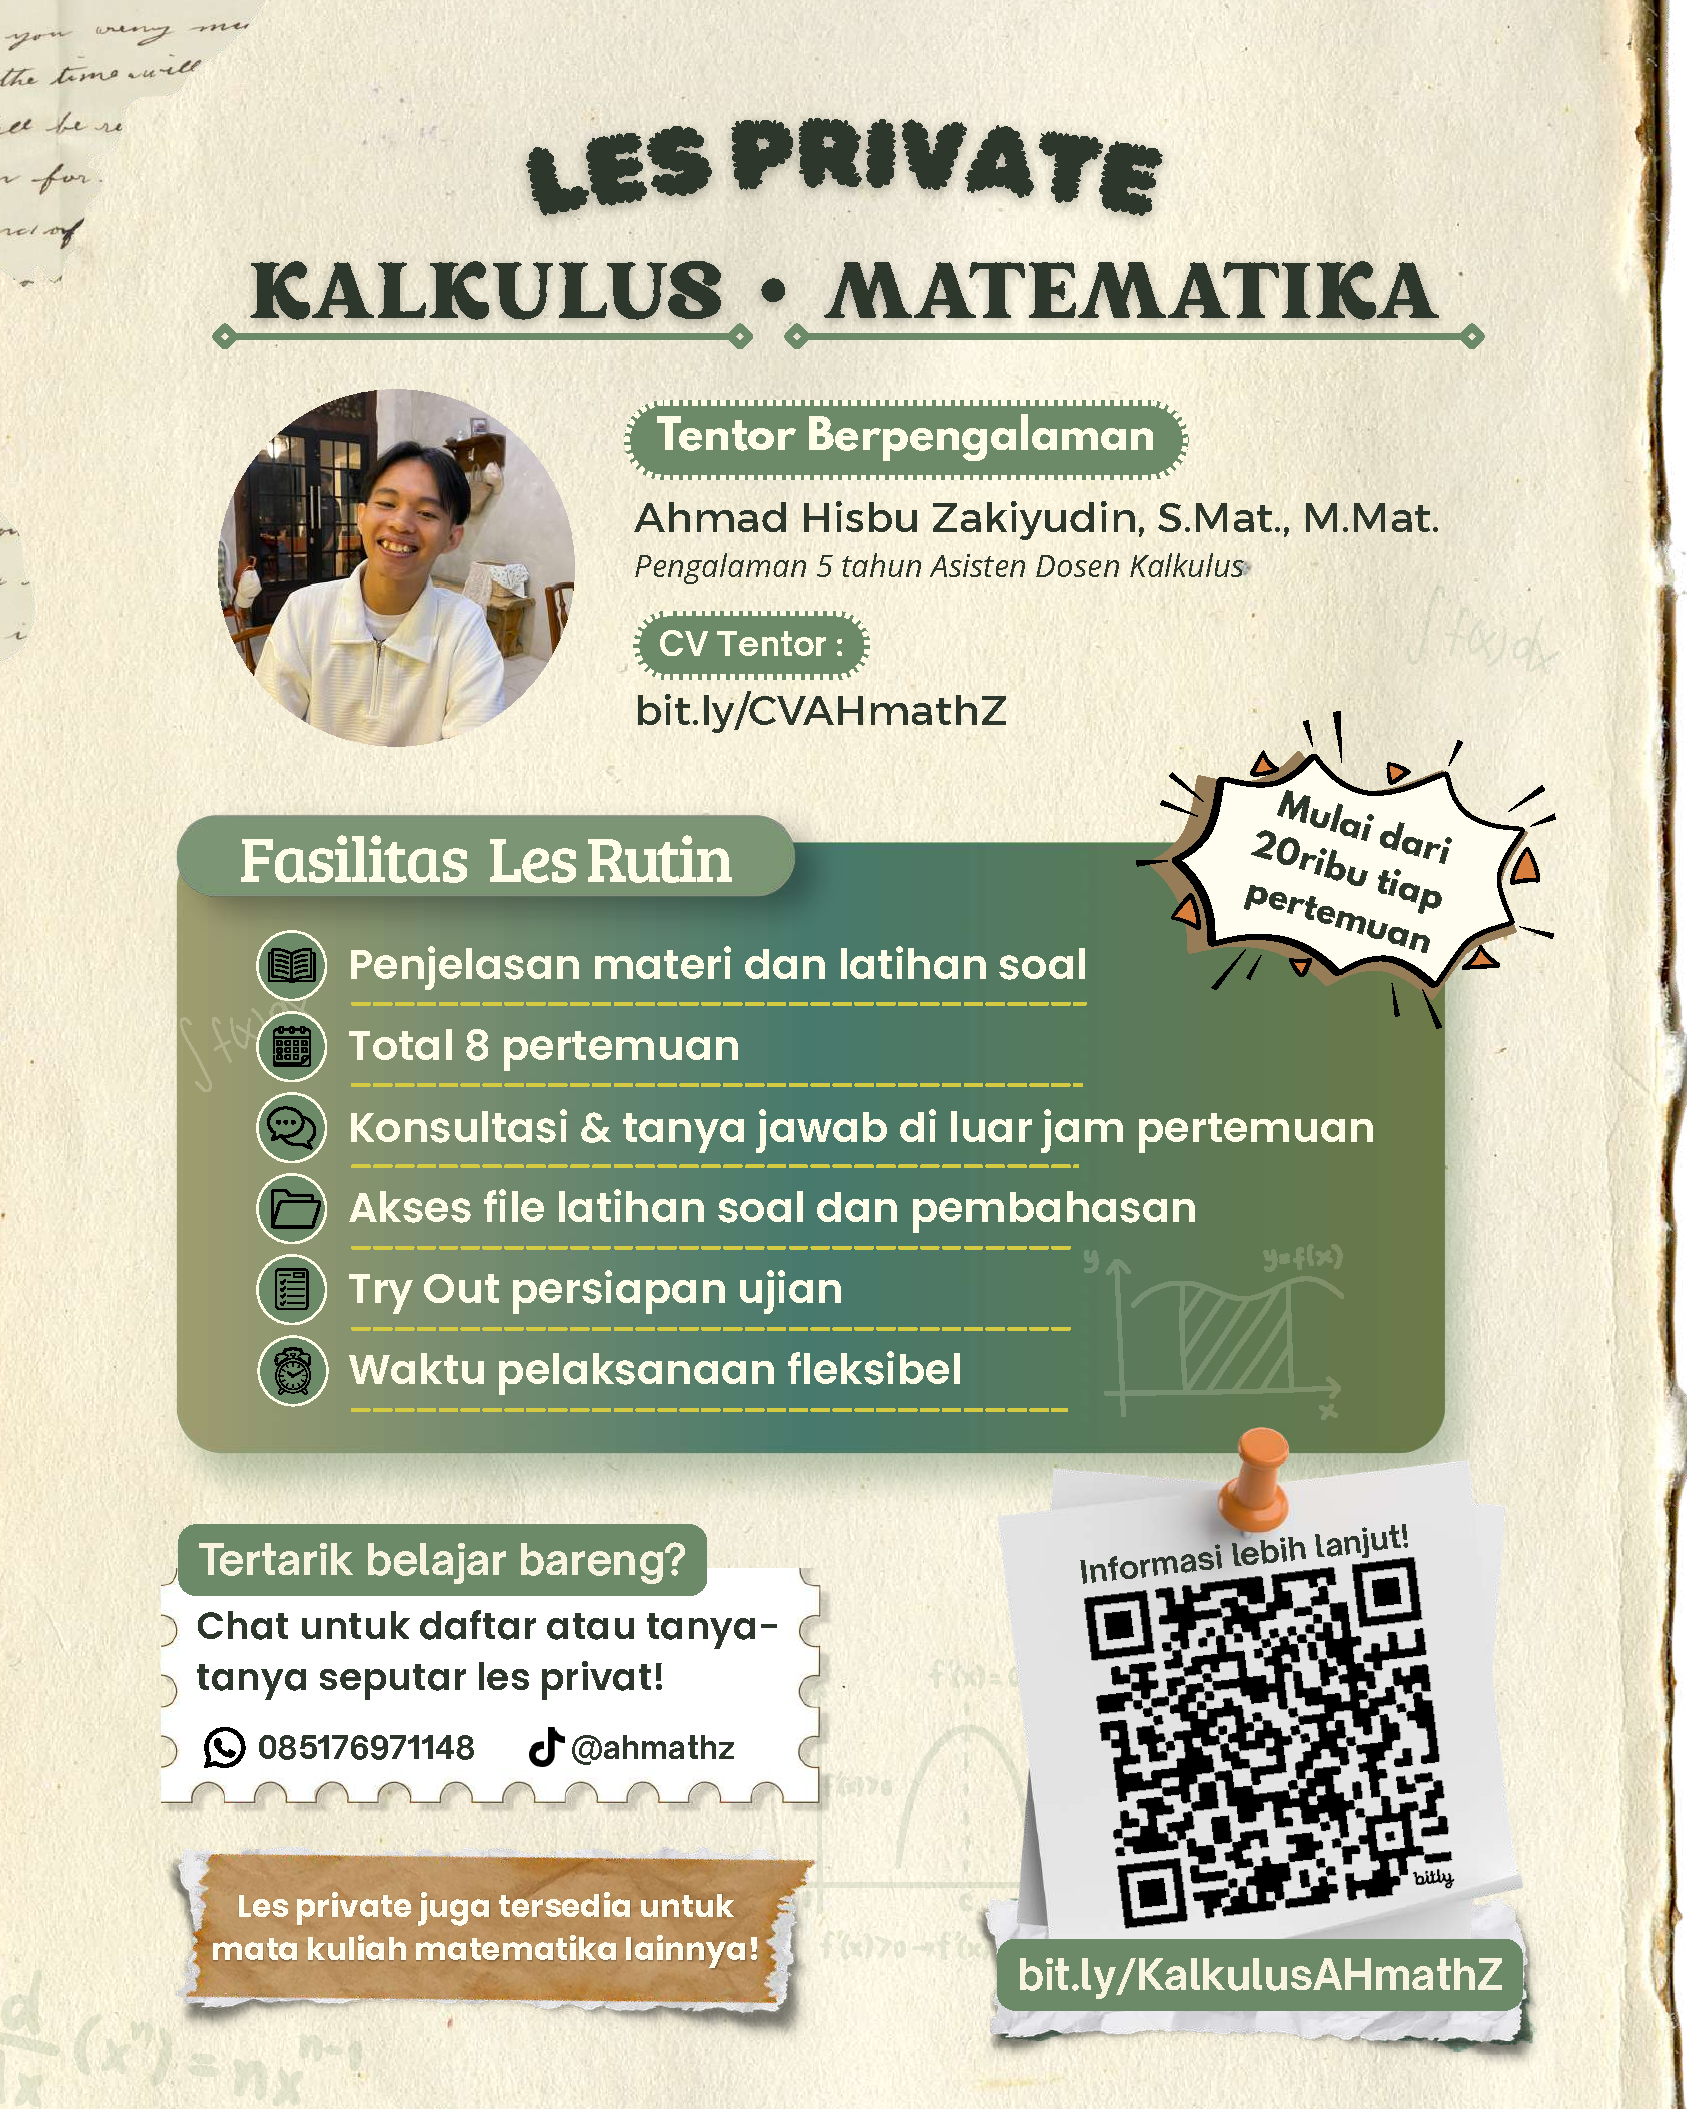
\includepdf[pages=-]{../ETS_Kalkulus_1_Th_2025-2026/les.pdf}

\end{document}
